


\chapter{week3}

\section{Tuesday}\index{Tuesday_lecture}
\subsection{Initial-boundary Value Problem}
Review:
\[\left\{\begin{gathered}u_{tt}=c^2\uxx\\u(x,0)=\varphi(x)\\u_t(x,0)=\psi(x)\\u(x,t)=\frac{1}{2}[\psi(x+ct)+\psi(x-ct)]+\frac{1}{2c}\int_{x-ct}^{x+ct}\psi(\xi)\diff \xi\end{gathered}\right.
\]
General solution: $u(x,t)=f(x+ct)+g(x-ct)$
\begin{figure}[H]
\centering
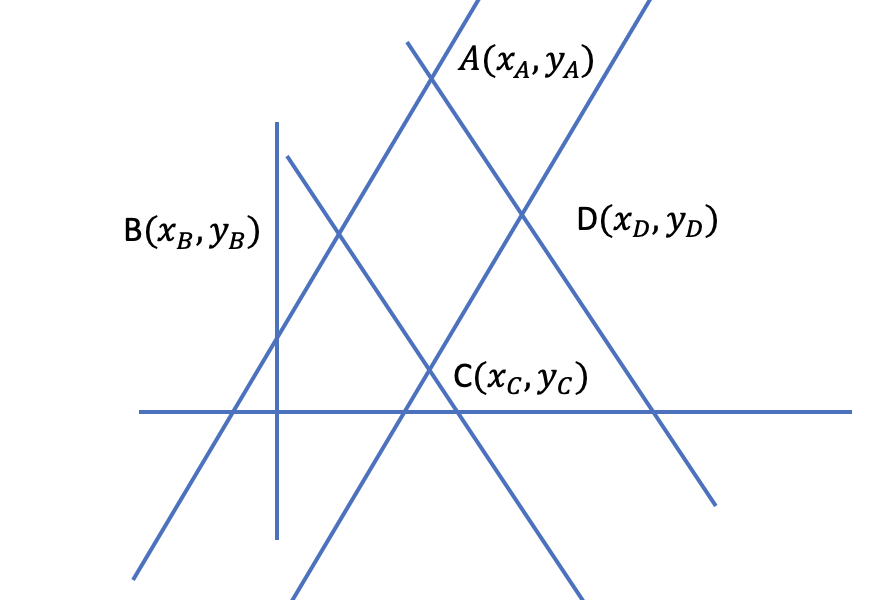
\includegraphics[width=4cm]{w2_th1}
\end{figure}

\[\left\{\begin{gathered}u_{tt}=c^2\uxx\quad x\in(0,L),~t\geq0\\
u(x,0)=\varphi(x)\quad x\in(0,L),~t\geq0\\
u_t(x,0)=\psi(x)\quad x\in(0,L),~t\geq0\\
u(0,t)=u(L,t)=0 \quad t\geq0\end{gathered}\right.
\]
\begin{figure}[H]
\centering
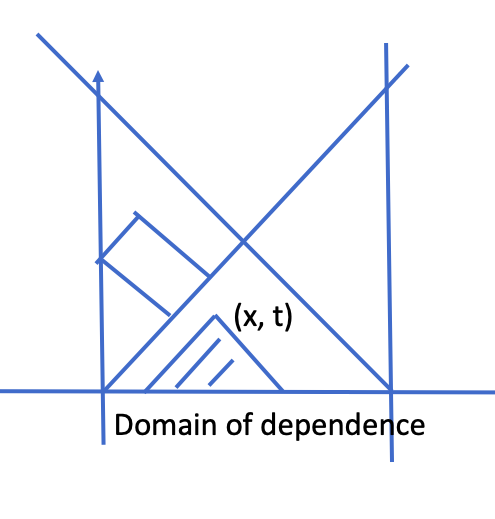
\includegraphics[width=8cm]{w3_tu}
\end{figure}

Assume
\[u(x,t)=X(x)T(t)
\]
\[u_{tt}=XT\pp
\]
\[\uxx=X\pp T
\]
\[XT\pp=c^2X\pp T
\]
\[\frac{T\pp}{c^2T}=\frac{X\pp}{X}=\lambda\text{  a constant}
\]
\[X\pp=\lambda X \quad\text{in } (0,L)
\]
Case (1): $\lambda=0$
\[X\pp=0
\]
\[X(x)=Ax+B
\]
\[X(0)=B=X(L)=AL=0\]
Case (2): $0<\lambda=\alpha^2$
\[\frac{X\pp}{X}=\alpha^2
\]
\[X(x)=c_1e^{\alpha x}+c_2e^{-\alpha x}
\]
\[X(0)=c_1+c_2=0
\]
\[X(L)=c_1e^{\alpha L}+c_2e^{-\alpha L}=0
\]
\[c_1e^{2\alpha L}+c_2=0
\]
\[c_1(e^{2\alpha L}-1)=0
\]
Similiarly, $c_2=0$\\
Case (3): $\lambda=-\beta^2<0$
\[\dakuohao{X\pp+\beta^2X=0}{X(0)=X(L)=0}
\]
\[X(x)=c_1\cos\beta x+c_2\sin\beta x
\]
\[X(0)=0=c_1
\]
\[X(L)=0=c_2\sin(\beta L)
\]
Want: $\beta L=n\pi$ , n=1, 2, 3,$\dots$
 $\beta=\frac{n\pi}{L}$, n=1, 2, 3, $\dots$
\[T\pp=-\beta^2c^2T
\]
\[T(t)=b_1\cos(\beta ct)+b_2\sin(\beta ct)=b_1\cos(\frac{n\pi}{L} ct)+b_2\sin(\frac{n\pi}{L} ct)
\]
As for any $n$, $u_n$ is a solution for ode, then for any linear combination of it, if it converges, is still a solution. We have:
\[u(x,t)=\sum_{n=1}^\infty[b_n\cos(\frac{n\pi}{L}ct)+c_n\sin(\frac{n\pi}{L}ct)]sin(\frac{n\pi}{L}x)
\]

Wish List:\\
(i) Converge for all $x, t$. In particular, it converges to $\varphi(x)$ when $t=0$\\
(ii)differentiable and converge to $\psi(x)$ when $t=0$\\
When $t=0$, $\psi(x)=u(x,0)=\sum_{n=1}^\infty b_n\sin(\frac{n\pi}{L} x)$. This series can converge to $\varphi$, as when $L=\pi$, $\{\sin x,\sin 2x, \sin 3x,\cdots,\sin nx,\cdots\}$ is a basis for the continuous function space with inner product $<f,g>=\frac{1}{L}\int_0^L fg(x)\diff x$. 





